%
% TikZ code to draw a (pseudo) Erdos-Renyi random graph
%
\documentclass[tikz]{standalone}

\usepackage[first=0,counter=rand]{lcg}% to generate (pseudo) random integers

\begin{document}
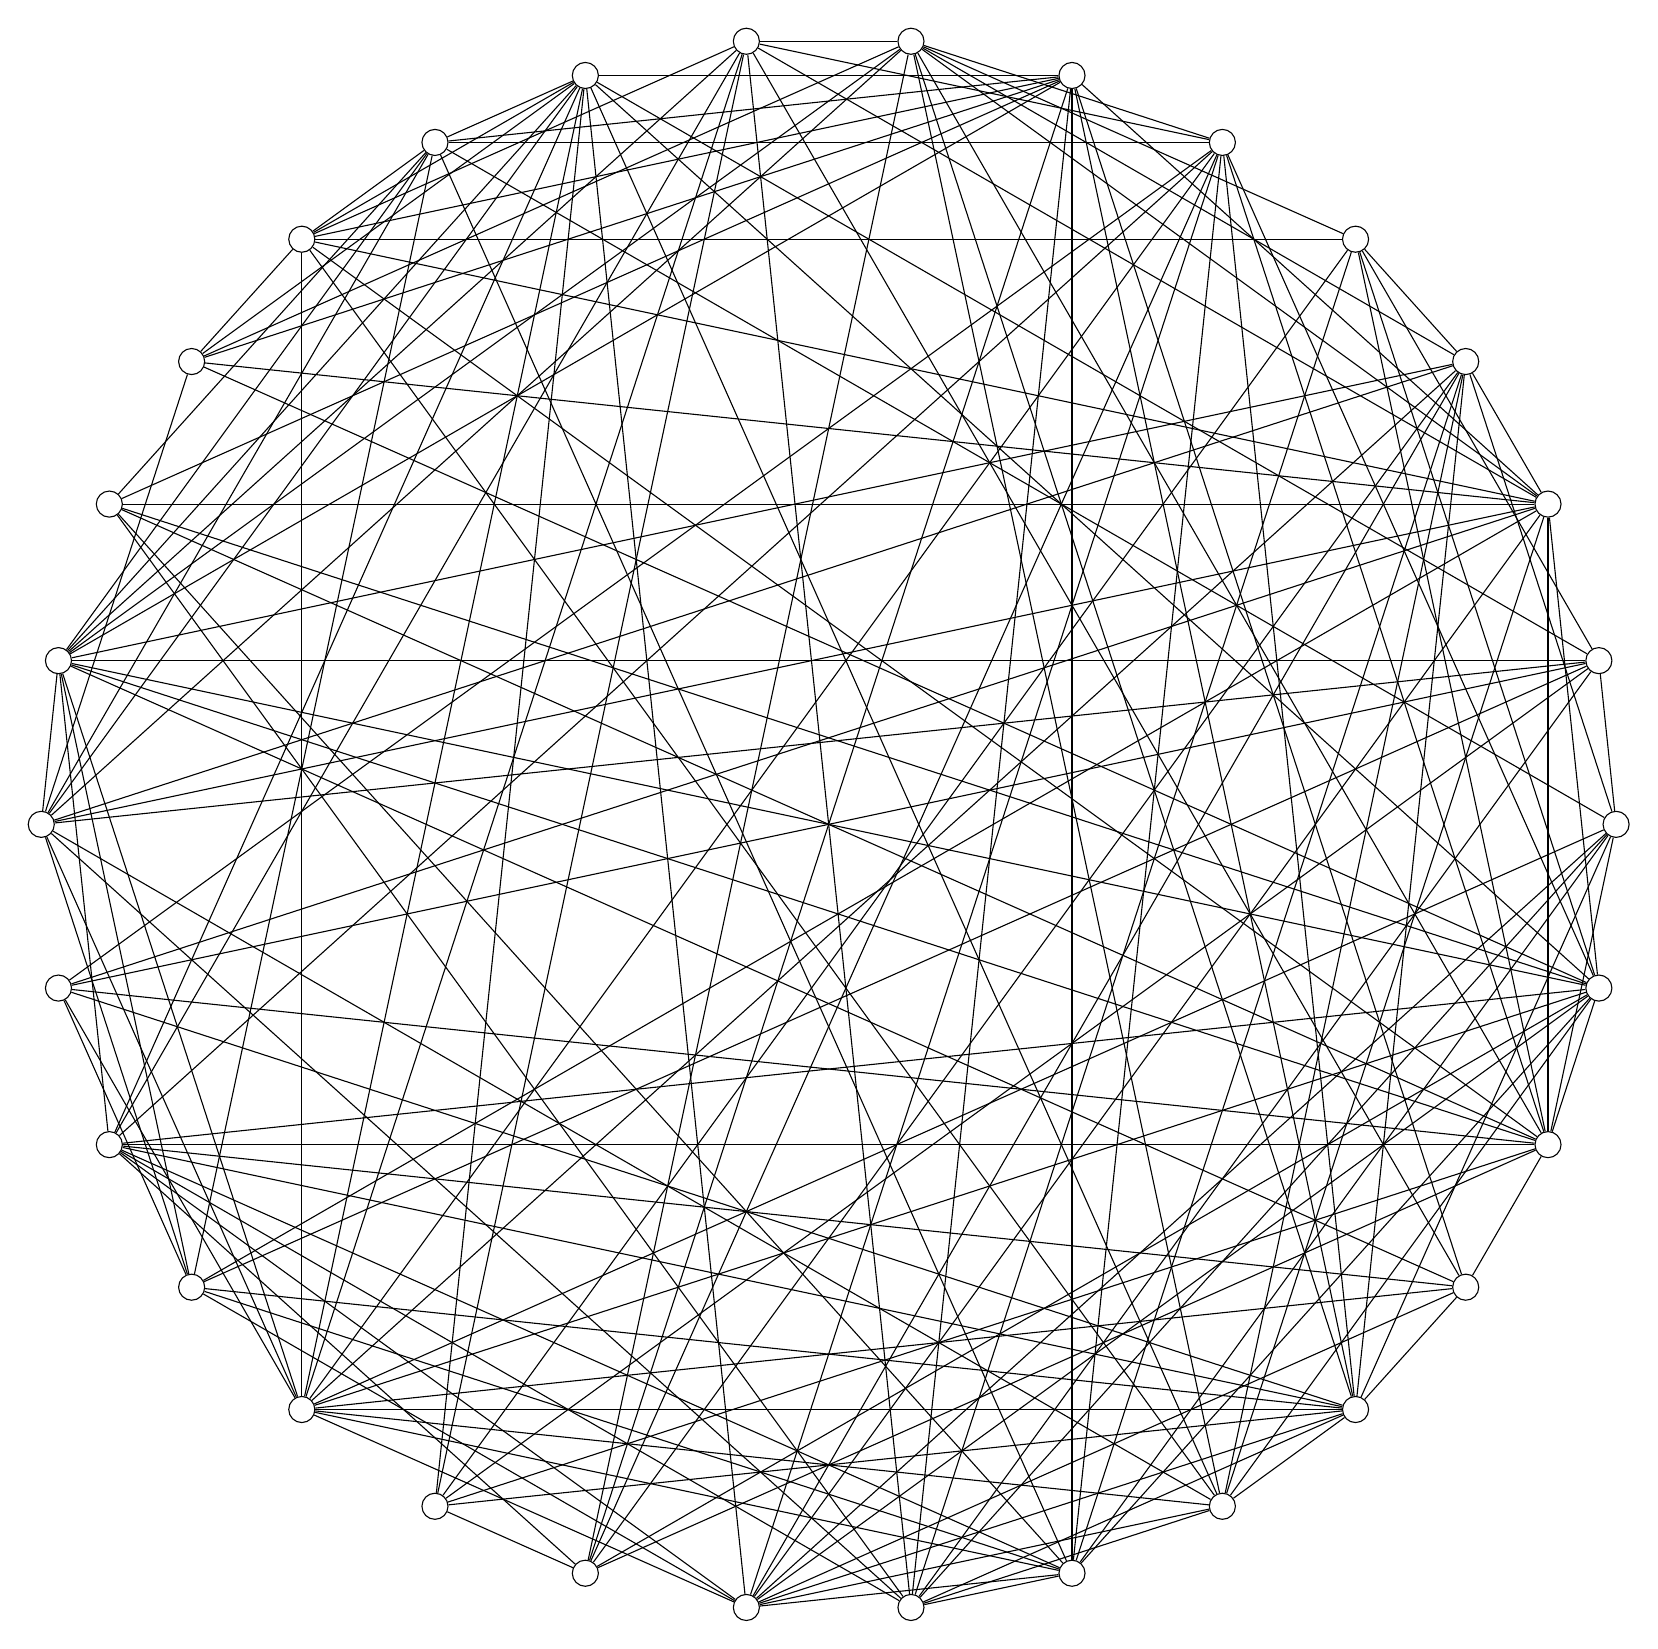
\begin{tikzpicture}

\def\n{30}					% number of nodes in the graph
\def\p{.3}					% edge density, the real edge density is not exactly \p. it is 1/(int(round(1/\p)))

%drawing parameters
\def\r{10cm}				% radius of the circle
\def\color{white}		% fill color for the nodes

\pgfmathsetmacro\range{int(round(1/\p))-1}
\chgrand[last=\range]


\foreach \i in {1,...,\n}{% draw the vertices
\pgfmathparse{360/\n*\i}%how the arithmetic is written here is *relevant*
\draw (\pgfmathresult : -\r) node[draw=black, circle, fill=\color] (\i){};
}

\foreach \i in {1,...,\n}{
\foreach \j in {\i,...,\n}{
\rand
\ifnum\arabic{rand}=0
\draw (\i) -- (\j);
\fi
}
}

\end{tikzpicture}	
\end{document}